% arara: lualatex: {shell: yes}

\documentclass[10pt]{article}

\usepackage{all-pairs-shortest-path-preamble}

\title{Resolvendo o problema do menor caminho}
\subtitle{Paralelização através MPI com o algoritmo de \emph{Fox}}
\author{Tarso Boudet Caldas \and up202204297}
\date{\today}

\subject{Computação Paralela}{CC4014}
\location{Porto}

\begin{document}

\maketitle

\section{Introdução}

O problema de encontrar o menor caminho (\emph{All pairs shortest path}) é aquele em que
buscamos o menor caminho entro quaisquer dois pares de nós em grafo direcionado. A
\cref{fig:grafo-input6} exemplifica o tipo de grafo que tratamos e a matriz que
usamos para representar este mesmo grafo, onde cada entrada \(M_{ij}\) é a distância
da aresta que vai do nó \(i\) ao nó \(j\).

\begin{figure}[htp]
	\centering
	\begin{minipage}{.4\linewidth}
		\centering
		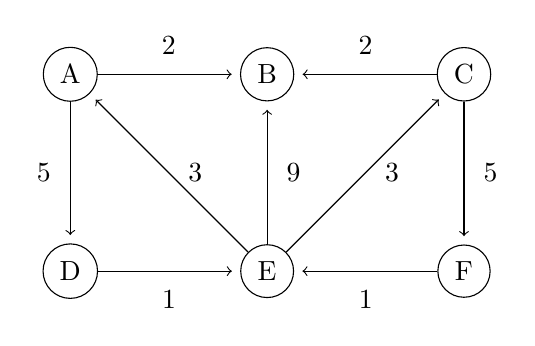
\begin{tikzpicture}[
				every path/.style = {->, shorten >= 3pt},
				every node /.style = {draw, circle, node distance = 6cm, inner sep = 3pt, minimum width = 3cm}
			]

			\node (a) [circle, draw] {A};
			\node (b) [right of = a, node distance = 2.5cm, circle, draw] {B};
			\node (c) [right of = b, node distance = 2.5cm, circle, draw] {C};
			\node (d) [below of = a, node distance = 2.5cm, circle, draw] {D};
			\node (e) [right of = d, node distance = 2.5cm, circle, draw] {E};
			\node (f) [right of = e, node distance = 2.5cm, circle, draw] {F};

			\path
			(a) edge node [label=above:{2}] {} (b)
			(a) edge node [label=left:{5}] {} (d)
			(c) edge node [label=above:{2}] {} (b)
			(c) edge node [label=right:{5}] {} (f)
			(d) edge node [label=below:{1}] {} (e)
			(e) edge node [label=right:{3}] {} (a)
			(e) edge node [label=right:{9}] {} (b)
			(e) edge node [label=right:{3}] {} (c)
			(f) edge node [label=below:{1}] {} (e);
		\end{tikzpicture}
	\end{minipage}
	\begin{minipage}{.4\linewidth}
		\centering
		\begin{equation*}
      M = 
			\begin{bmatrix}
				0 & 2 & 0 & 5 & 0 & 0 \\
				0 & 0 & 0 & 0 & 0 & 0 \\
				0 & 2 & 0 & 0 & 0 & 5 \\
				0 & 0 & 0 & 0 & 1 & 0 \\
				3 & 9 & 3 & 0 & 0 & 0 \\
				0 & 0 & 0 & 0 & 1 & 0
			\end{bmatrix}
		\end{equation*}
	\end{minipage}
	\caption{Grafo direcionado com valores atribuídos para cada aresta e a matriz quadrada correspondente.}%
	\label{fig:grafo-input6}
\end{figure}

A solução deste problema é também uma matriz quadrada, onde cada entrada \(N_{ij}\) é o disância do menor caminho
possível a ser percorrida para ir do nó \(i\) ao \(j\).

\[N = 
\begin{bmatrix}
	0 & 2 & 9 & 5  & 6 & 14 \\
	0 & 0 & 0 & 0  & 0 & 0  \\
	9 & 2 & 0 & 14 & 6 & 5  \\
	4 & 6 & 4 & 0  & 1 & 9  \\
	3 & 5 & 3 & 8  & 0 & 8  \\
	4 & 6 & 4 & 9  & 1 & 0
\end{bmatrix}
\]

Neste trabalho, iremos descrever uma solução para este problema adotando paralelismo através de \ac{mpi} usando
o \emph{algoritmo de Fox}, distribuindo processos entre diversas configurações de máquinas e os organizando 
em um comunicador de \emph{grid}.

\section{Solucionando o problema}

Para encontrar a matriz \(N\) dos menores caminhos a partir de \(M\), 
elevar \(M\) ao quadrado sucessivamente até que \(N = M^{2^{\log(n-1)}}\),
onde \(n\) é o número de nós do grafo. Para isso, implementamos o seguinte
algoritmo de multiplicação de matrizes apresentado no
\cref{lst:matrix-multiply}.

\begin{listing}
\cfile[firstline=54, lastline=69]{../mtrxop.c}
\caption{Algoritmo de multiplicação de matrizes no arquivo \file{mtrxop.c}.}
\label{lst:matrix-multiply}
\end{listing}

O que difere este algoritmo de uma multiplicação é 
que em vez de multiplicar as entradas \(A_{i,k}\) e
\(B_{k,j}\), com \(k=1,\ldots,n\), e somar os respectivos
\(k\) resultados, somamos \(A_{i,k}\) com \(B_{i,k}\) e
escolhemos os menor resultado (ignorando as entradas com 
valor 0). Com isso encontramos o \emph{produto da distância}
entre duas matrizes, e repetindo este processo sucessivamente,
até \(M^{n-1}\), encontramos a matriz de distância, e portanto,
resolvemos o problema.

\section{Paralelizando a multiplicação através do algoritmo de Fox}

O \emph{algoritmo de Fox} nos permite dividir a tarefa de multiplicação
da matriz em diversos processos fazendo multiplicações de matrizes menores
em cada um. Para isso, dividimos a matriz em um \emph{grid}, isto é,
uma malha com divisões iguais ao número de processos. Por exemplo,
na matriz \(M\), poderiamos ter

\[
	M_0 =
	\begin{bmatrix}
		0 & 2 & 9 \\
		0 & 0 & 0 \\
		9 & 2 & 0
	\end{bmatrix},\quad
	M_1 =
	\begin{bmatrix}
		5  & 6 & 14 \\
		0  & 0 & 0  \\
		14 & 6 & 5
	\end{bmatrix},\quad
	M_2 =
	\begin{bmatrix}
		4 & 6 & 4 \\
		3 & 5 & 3 \\
		4 & 6 & 4
	\end{bmatrix},
	M_3 =
	\begin{bmatrix}
		0 & 1 & 9 \\
		8 & 0 & 8 \\
		9 & 1 & 0
	\end{bmatrix}.
\]

Com \ac{mpi}, podemos definir o grid como um \emph{struct}
\cinline/GRID_TYPE/, como mostra o \cref{lst:grid-type}. O grid que criamos deve possuir
dimensão \(q\timesq\), onde \(q=\sqrt{p}\) e \(p\) é o número de processos. Dizemos
que \(q\) é a \emph{ordem} do \emph{grid}.

\begin{listing}
	\cfile[firstline = 6, lastline = 15]{../mtrxop.h}
	\caption{Definição do tipo \cinline/GRID_TYPE/ no arquivo \file{mtrxop.h}}%
	\label{lst:grid-type}
\end{listing}

Aqui definimos três comunicadores, um para o grid, um para linhas e outro para colunas,
além de definirmos o número de processos, a ordem  do grid, além de ter a informação
da linha e coluna no grid. Usamos então para inicar o \emph{grid} a função \cinline{setupGrid(GRID_TYPE)}, %chktex 36
definida no \cref{lst:setup-grid}.

\begin{listing}
	\cfile[firstline=85,lastline=105]{../mtrxop.c}
	\caption{Inicialização do \emph{grid} definida em \file{mtrxop.c}.}%
	\label{lst:setup-grid}
\end{listing}

Por fim, definimos no \cref{lst:fox} função que aplica o algoritmo de Fox para
efetuar a multiplicação de matrizes. Este algoritmo escolhe uma submatriz \(A\) de
cada linha e a envia para os outros processos daquela linha, e então cada processo
multiplica a matriz recebida com uma matriz \(B\) presente previamente (inicialmente 
igual a \(A\)). Cada processo então envia a matriz \(B\) para o processo acima no \emph{grid}.

\begin{listing}
	\cfile[firstline=108,lastline=127]{../mtrxop.c}
	\caption{Algoritmo de Fox.}%
	\label{lst:fox}
\end{listing}

\pagebreak

\section{Execução do programa}

Para executar o programa, basta compilar o projeto usando \verb|make|, e então
executar como seguem as instruções no \cref{lst:help}

\begin{listing}
  \small
	\begin{verbatim}
  Usage: mpirun -np <processes> shortest-path [options]
      -i <file> --input <file>    Set matrix input file
      -o <file> --output <file>   Specify custom output name
      -h --help                   Display this help message
      -t --timing-only            Don't print the solution, only the timing
      -r --random-matrix <size>   Use random matrix as input
                                  (only if no input file provided)
  \end{verbatim}
	\caption{Funcionalidade do programa \file{shortest-path}.}%
	\label{lst:help}
\end{listing}

É necessário que o número de processos seja um quadrado perfeito, a fim de
que estes possam ser organizados em um \emph{grid}.

Podemos rodar o programa tanto utilizando um arquivo com uma matriz em
que a primeira linha contém o número de nós do grafo, ou então gerar uma matriz
aleatória de tamanho arbitrário. Em ambos os casos, as matrizes planificadas
em um \emph{array} \cinline{totalMatrix[]} de tamanho \(n\times n\), que é então populado nas matrizes
\(A\) de cada processo através de \cinline{MPI_Scatter()}. %chktex 36
Compiamos então a matriz \(A\) para \(b\) e \(C\), e podemos
aplicar o algoritmo de Fox até que tenhamos a matriz de distância, 
como ilustra o \cref{lst:fox-loop}.

\begin{listing}
  \cfile[firstline=155, lastline = 165]{../main.c}
  \caption{Loop do algoritmo Fox sobre as matrizes \(A\) e \(B\) de cada processo.}%
  \label{lst:fox-loop}
\end{listing}

Terminamos usamos \cinline{MPI_Gather()} para copiar as matrizes de volta %chktex 36
para o array \cinline{totalMatrix[]} e temos o nosso resultado.

\section{Análise de performance}

Para analisar a o desempenho deste programa, o rodamos com diferentes configurações de matrizes,
de processos e número de máquinas em comunicação. Cada configuração foi corrida 50 vezes
através de um script, e foram registrados o tempo de cada corrida através de
\cinline{MPI_Wait()}  e também registrado o tempo total de rodar as 50 vezes.%chktex 36
No primeiro caso, não é incluída o tempo de comunicação entre as máquinas, portanto
é possível registrar o tempo de execução do processo em si, como também a diferença
de tempo de comunicação. Nos gráficos da \cref{fig:timing-graphs} temos o resultado de tempo.

\begin{figure}[htp]
  \centering
	\begin{minipage}{.49\linewidth}
    \begin{SubFloat}{Tempos de matrizes de ordem 6.\label{fig:timings6}}
			\includestandalone{./tikz/matrix6}
		\end{SubFloat}
	\end{minipage}
	\begin{minipage}{.49\linewidth}
    \begin{SubFloat}{Tempos de matrizes de ordem 300.\label{fig:timings300}}
			\includestandalone{./tikz/matrix300}
		\end{SubFloat}
	\end{minipage}

	\begin{minipage}{.7\linewidth}
    \begin{SubFloat}{Tempos de matrizes de ordem 600.\label{fig:timings600}}
			\includestandalone{./tikz/matrix600}
		\end{SubFloat}
	\end{minipage}

	\begin{minipage}{.7\linewidth}
    \begin{SubFloat}{Tempos de matrizes de ordem 900.\label{fig:timings900}}
			\includestandalone{./tikz/matrix900}
		\end{SubFloat}
	\end{minipage}
  \caption{\small
    Gráficos com os tempos das matrizes. Os pontos vermelhos representam as médias tempo de resolução 
    do problema já com a comunicação iniciada, e os pontos azuis as médias de tempo execução da chamada
    de \file{mpirun} 50 vezes. No eixo \(x\) temos as configurações das máquinas no formado \(c_i=(m;p)\),
    onde \(m\) representa o número de máquinas usadas e \(p\) o de processos. As configurações
    com \enquote{\(*\)} indicam que a distribuição dos processos entre as máquinas não é balanceada.
  }\label{fig:timing-graphs}
\end{figure}

A partir dos gráficos, é possível analisar que para matrizes pequenas como na \cref{fig:timings6},
a paralelização não faz tanto sentido, já que a diferença de tempo é negativa, quanto mais processos 
e máquinas utilizamos para resolver o problema, visto que o tempo de comunicação do \ac{mpi} é o 
gargalo da aplicação.

A diferença passa a ser perceptível (mas ainda tímida) quando olhamos os casos das matrizes de 300 nós, 
onde o uso de 4 processos em uma máquina é quase \(\frac{1}{4}\) do de um processo, mas é possível
observar que distribuir estes processos entre um número maior de máquinas cria um \emph{overhead}
significativo, o que nos leva a crer que é preferível rodar os processos em um número menor
de máquinas possível. No gráfico da \cref{fig:timings300}, o melhor resultado é quando usamos
16 processos, mas apenas quando são executados em duas máquinas, e ainda assim, o tempo total
de execução foi maior neste caso do que quando se usam 9 processos. Os casos de 9 processos
são notáveis, pois contradiz a observação feita anteriormente, pois o melhor resultado é dividindo
em 3 máquinas em vez de duas, onde ambas configurações \(c_i=[p_1,\ldots,p_m]\), do número de processos da máquina
\(i\) foram \(c_7=[4,5]\) (uma máquina com 4 processos e outra com 5) e \(c_7=[8,1]\), respectivamente, 
e a diferença é pouco notável entre os três casos, apesar de \(c_5\) possuir uma vantagem sobre 
\(c_5=(3;9)\) no tempo de execução do processo, o tempo total de execução de \(c_5\) foi ligeiramente
melhor.

É muito mais considerável a diferença entre um e mais processos  chegamos a matrizes de ordem
600, onde 1 processo demora seis vezes mais do que 4 em uma máquina. Também vemos na 
\cref{fig:timings600} que \(c_8=(2;16)\) continua a ser dar o melhor 
resultado na resolução, e isto também se repente nas matrizes de ordem 900. É mais 
considerável no caso de 600 nós do que no de 300 a discrepância na duração do
programa quando introduzimos mais máquinas e mantemos o número de processos, com 
uma importante exceção que é quando temos \(c_{12} = (6;36)\), que consegue
ter vantagem sobre a configuração com estes processos distribuídos em apenas 5,
que é o caso de \(c_{13} = [8,8,8,8,4]\). Isto talvez ocorra pois \(c_{12}\) 
se enquadra melhor na definição do comunicador em \emph{grid}.

O gráfico da \cref{fig:timings900} possui a mesma tendência do anterior,
sua principal variação é que em matrizes maiores, aumentar o número de processos
após 16 não cria um \emph{overhead} tão considerável, possivelmente pois
o tempo de processamento em si começa a alcançar o \emph{bottleneck} 
dos comunicadores. É possível que se passarmos a lidar com matrizes ainda 
maiores, configuração com um número de processadores maiores consigam 
term um melhor desempenho do que a configuração \(c_8\).

\section{Conclusão}

Com este trabalho foi possível chegar à conclusão que o tamanho do problema é fundamental quando queremos
encontrar o ponto ótimo de eficiência da distribuição de processos usando \ac{mpi}. Quando o problema
é pequeno demais, o custo da comunicação não compensa as possíveis vantagens do paralelismo, e mesmo
quando consideramos problemas maiores, nem sempre mais máquinas ou mais processos significa uma melhoria
no tempo de execução. Por este motivo, antes de se decidir uma configuração para executar um programa em
paralelo, é sempre importante ter os \emph{benchmarks} adequados para o tipo e tamanho de problema que estamos
lidando.


% \nocite{*}
\printbibliography

\end{document}
